\section{Data}
% Describe how you explored your data, and the process through which you determined your
% input features. How did you end up representing your data? What else did you try? We are looking for:
% – A thorough exploration of the data, similar to what is presented in labs. What are the distributions of the features? How do these features correlate with the target?


% – If you use figures to answer those questions, an explanation of how you are interpreting those figures. Take care that your figures can be interpreted meaningfully.

% – A clear and logical description of how you determined your input features, with convincing logical or empirical evidence justifying your choice. Important features are not overlooked (e.g., not removed for “ease”).
% – A clear description of the way(s) that you are representing the data in your models.
% – The descriptions should be consistent with the .py and/or .ipynb files that you used while developing your model.
% – A clear description of how you are splitting your data into various sets. You may use k-fold cross validation if you’d like, but if you do, describe how you are applying that idea.


% id,"Q1: From a scale 1 to 5, how complex is it to make this food? (Where 1 is the most simple, and 5 is the most complex)",
% Q2: How many ingredients would you expect this food item to contain?,
% Q3: In what setting would you expect this food to be served? Please check all that apply,
% Q4: How much would you expect to pay for one serving of this food item?,
% Q5: What movie do you think of when thinking of this food item?,
% Q6: What drink would you pair with this food item?,"
% Q7: When you think about this food item, who does it remind you of?",
% Q8: How much hot sauce would you add to this food item?,Label

\subsection{Cleaning}
\label{sec:cleaning}
The multiple-choice questions (Q1, Q3, Q7, Q8) were split into individual one-hot features, and Q3 & Q7, which both allowed multiple answers, also had each combination represented as a one-hot feature (if they appear in the training data at least 5 times) alongside a feature that represented the number of selected answers.

Q2 and Q4 were converted into numbers using the following logic:
\begin{itemize}
    \item If there is a range (two numbers with the word “to”, “and” or “-” between), then take the average
    \item Otherwise, take the first number that appears (it can handle numeric, and also written numbers up to 20)
    \item Otherwise, if it's the ingredients question, take the number of commas or line breaks, plus one
    \item Otherwise, return the average seen in the training
\end{itemize}

Q5 and Q6 were more complicated free-form text answers. To generalize as broadly to any input, we used a fuzzing library to cluster similar responses into singular features, assuming they appeared frequently enough in the training set. Then, for movie answers we only allowed a singular matched movie (or if nothing matched, “other”), but for drink answers multiple drinks could be listed.

Another approach we adopted was using a word2vec model on the free-form questionnaire responses. Word2vec learns vector representations for words, assigning similar embeddings to words with related meanings. This captures semantic relationships in the text and allows distances between embeddings to quantify word similarity. For each free-form answer and label (pizza, sushi, shawarma), we calculated the average word vector. Each question had three features, one per food type, that recorded the cosine similarity between the free-form answer's averaged vector and the averaged vector for each label.

This was all condensed into a function that took in a CSV file, split the data as needed, and output a dataframe of the flattened vectors for every feature.


\subsection{Exploration}
\label{sec:exploration}
We visualized the cleaned data using histograms and boxplots to explore the data. Some questions such as Q3: "In what setting 
would you expect this food to be served?" have multiple choice as inputs, and others such as Q5: "What movie do you think of when thinking of this food item?"
allow participants to type their responses. For those questions, we counted the number of occurrence for each input, and only show the top 5 responses in the graph 
so it is readable while capturing the most important information.

% Q1
Figure \ref{f:hist_q1} shows a histogram of responses for Q1: From a scale 1 to 5, how complex is it to make this food?. For Sushi, 
the difficulty is generally higher with more inputs of 4 and 5. For Pizza, we see medium complexity(3) being the highest choice. For Shawarma,
we see more votes in the range of 4 and 5.
\begin{figure}[h]
    \centerline{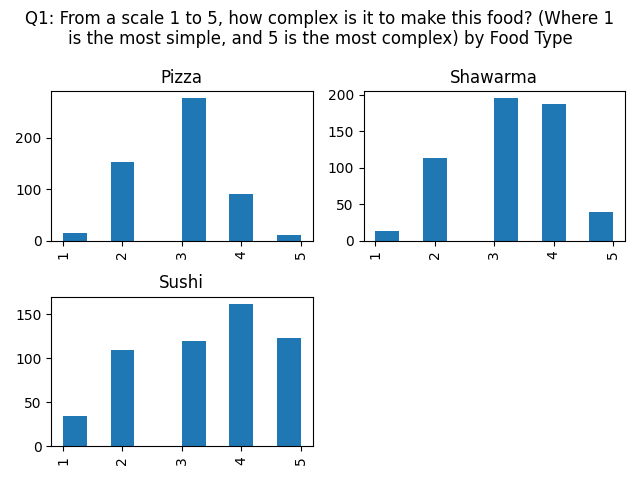
\includegraphics[width=\columnwidth]{data/histogram_Q1.png}}
    \caption{Histogram for Q1: How complex is it to make the food}
    \label{f:hist_q1}
\end{figure}


% Q2
In figure \ref{f:box_q2}, the boxplot illustrates the distribution of expected ingredient counts for each food class. 
We see the participants generally expect the fewest ingredients in Sushi (median ~4), 
followed by Pizza (median ~5), and then Shawarma (median ~7). Shawarma shows the greatest variability in expected ingredient 
counts, while Pizza and Sushi show less variability. All three food types have outliers, suggesting some individuals expect 
significantly more ingredients than the majority. We see in \ref{f:hist_q2} that the histograms shows a right-skewed distribution 
for all three food items, indicating most respondents expect a low number of ingredients. 
However, the skewed pattern suggests a minority of participants anticipate a considerably higher ingredient count.

\begin{figure}[h]
    \centerline{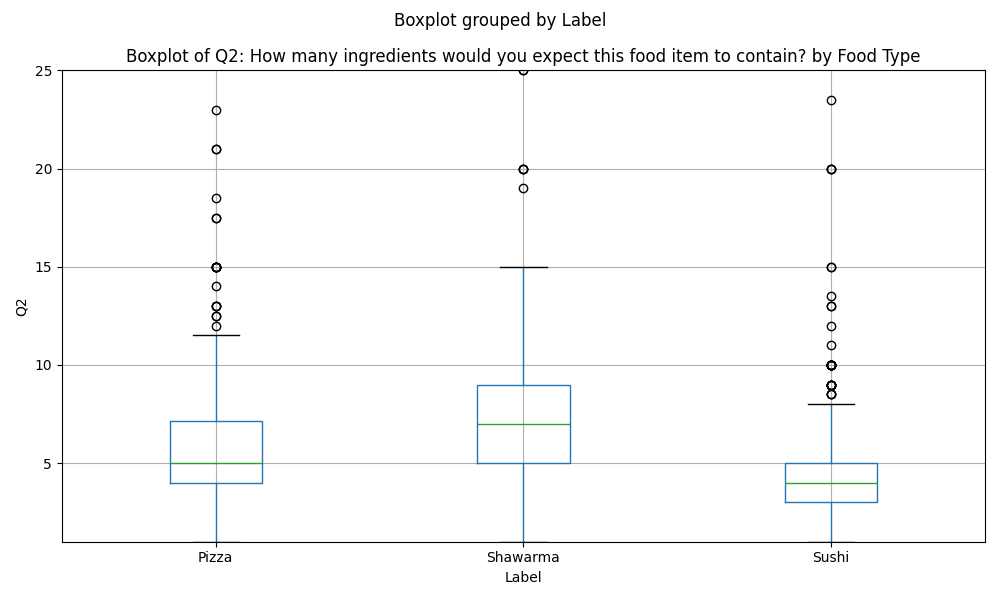
\includegraphics[width=\columnwidth]{data/boxplot_Q2.png}}
    \caption{Boxplot for Q2: How many ingredients would you expect the food to have}
    \label{f:box_q2}
\end{figure}

\begin{figure}[h]
    \centerline{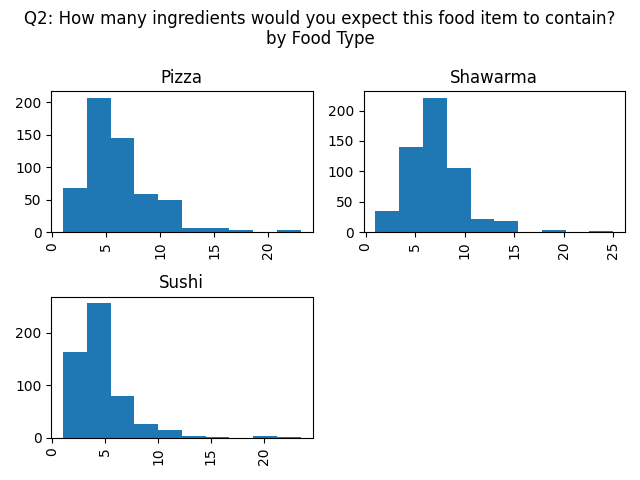
\includegraphics[width=\columnwidth]{data/histogram_Q2.png}}
    \caption{Histogram for Q2: How many ingredients would you expect the food to have}
    \label{f:hist_q2}
\end{figure}

% Q3 TODO the graph is annoying
Question 3 is "In what setting would you expect this food to be served?". 
For Q3: “In what setting would you expect this food to be served?”, we see a trend that Pizza is more appropriate for most situations, and shawarma and sushi are more specific in when they are expected to be served.


% Q4 

In figure \ref{f:hist_q4}, we see a majority of participants expecting to pay a lower price for the food. 
Interestingly we see much higher outliers for sushi, with a peak of someone willing to pay ~100 dollars 
for one serving of sushi. We also see different distributions for the three food items - pizza has a peak at 
~5 dollars, with a tail towards higher prices; shawarma has a normal distribution with mean at ~10 dollars.
\begin{figure}[h]
    \centerline{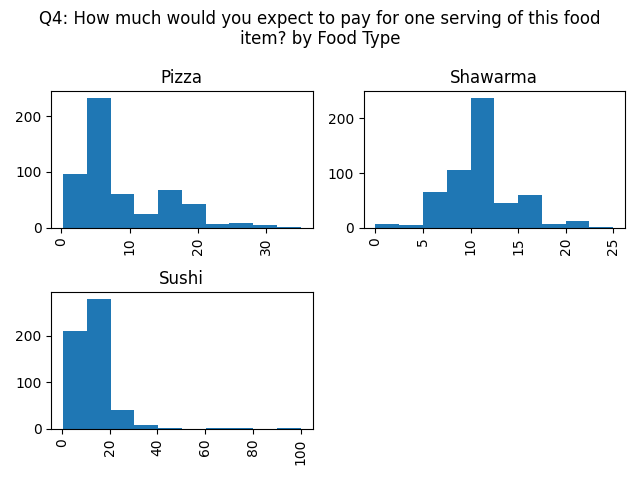
\includegraphics[width=\columnwidth]{data/histogram_Q4.png}}
    \caption{Histogram for Q4: How much would you expect to pay for one serving of this food item?}
    \label{f:hist_q4}
\end{figure}

% Q5 What movie do you think of when thinking of this food item?
Figure \ref{f:pizza_q5}, \ref{f:shawarma_q6}, \ref{f:sushi_q5} shows the top responses for each class for Q5.
For both Pizza and Sushi, we saw “none” as the most popular input. However for Shawarma we saw “Avengers” to be by far the most popular response for Shawarma, suggesting a 
correlation between "Avengers" and "Shawarma", making Q5 a good indicator.

\begin{figure}[ht]
    \centerline{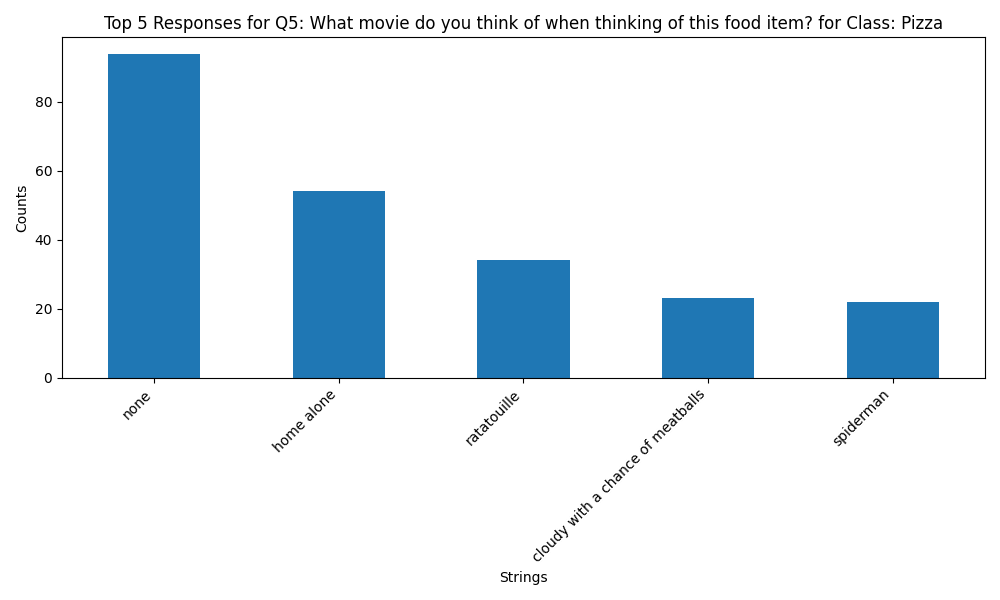
\includegraphics[width=\columnwidth]{data/top_5_responses_Q5_Pizza.png}}
    \caption{Counts for Pizza for Q5: What movie do you think of when thinking of this food item?}
    \label{f:pizza_q5}
\end{figure}

\begin{figure}[ht]
    \centerline{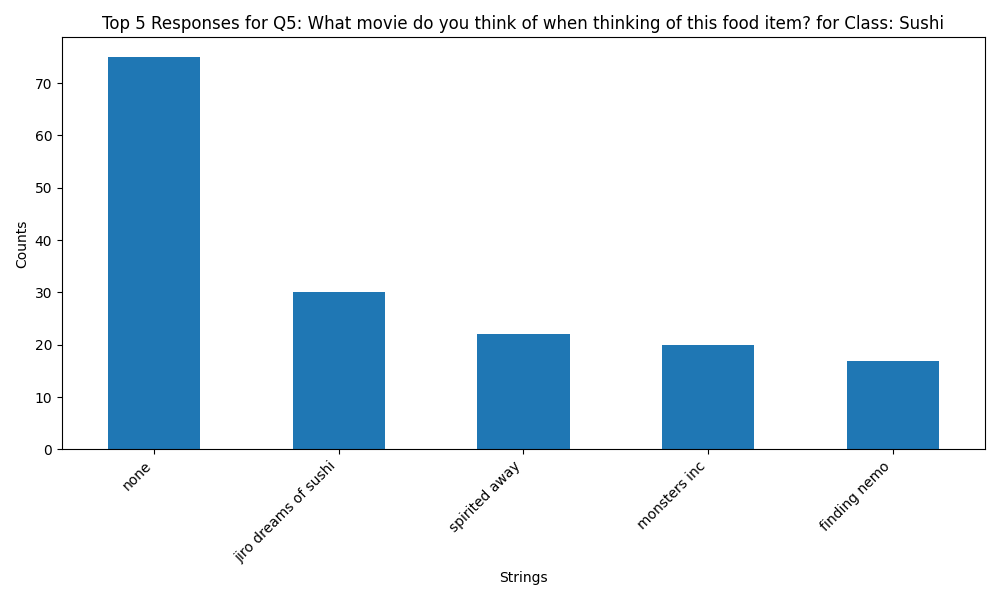
\includegraphics[width=\columnwidth]{data/top_5_responses_Q5_Sushi.png}}
    \caption{Counts for Sushi for Q5: What movie do you think of when thinking of this food item?}
    \label{f:sushi_q5}
\end{figure}
\begin{figure}[ht]
    \centerline{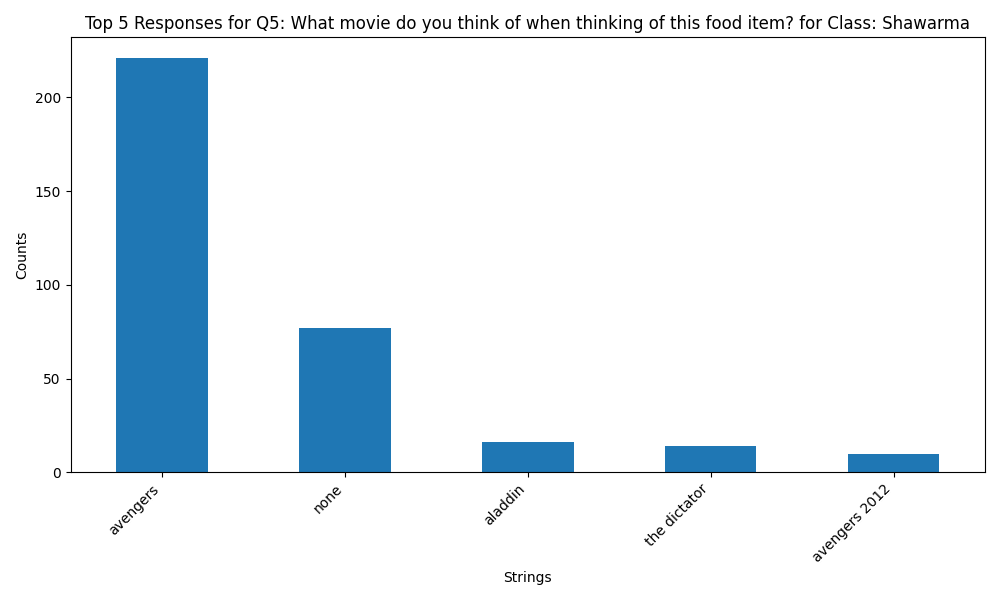
\includegraphics[width=\columnwidth]{data/top_5_responses_Q5_Shawarma.png}}
    \caption{Counts for Shawarma for Q5: What movie do you think of when thinking of this food item?}
    \label{f:shawarma_q6}
\end{figure}


%Q6
For Q6: "What drink would you pair with this food item?" we see a substainal difference between the answers for the three foods.
With sushi participants preffered water, tea or sake. With Piazza there was a clear prefference for Cock-cola and other fizzy drinks
and Shawarma had a tie between water and coca cola for the most frequent response with a siginficant minority preffering juice or
nothing at all.

\begin{figure}[ht]
    \centerline{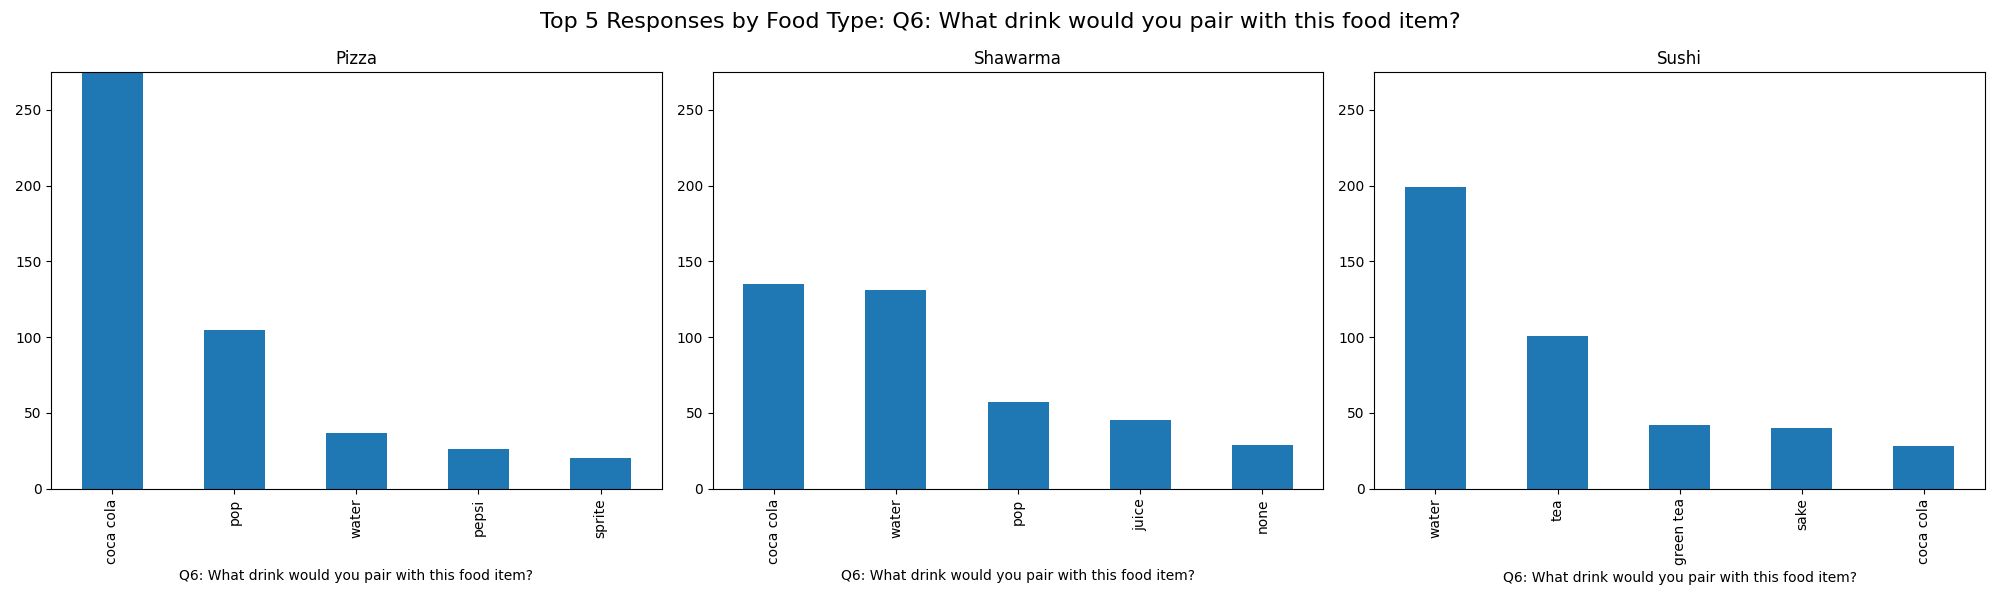
\includegraphics[width=\columnwidth]{data/top_5_responses_Q6.png}}
    \caption{Top 5 Responses for Q6}
    \label{f:q6}
\end{figure}

%Q7
With regards to Q7: “when you think about this food item, who does this remind you of?”, there are no clear indicating responses
between the food classes. For example, the most popular response accross the three foods for Q7 was “Friends”, with the remaining
responses being, similar in size and frequency across the three food items. Therefore we decided to remove this Q7 from the parameters. 

\begin{figure}[ht]
    \centerline{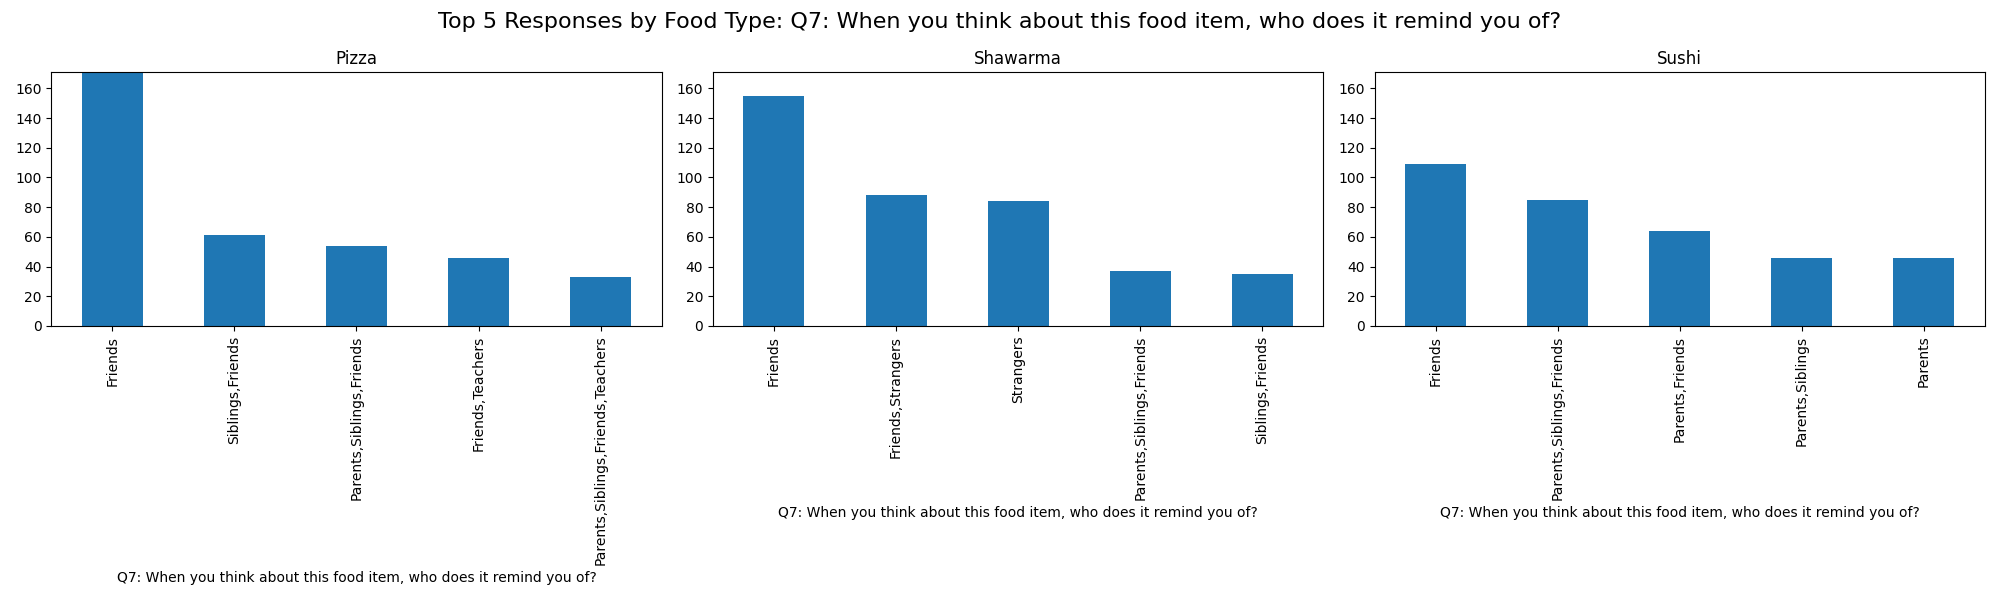
\includegraphics[width=\columnwidth]{data/top_5_responses_Q7.png}}
    \caption{Top 5 Responses for Q7}
    \label{f:q7}
\end{figure}

We split the dataset into 3 sets: 60\% training, 20\% validation and 20\% test. This allowed us sufficient data to train the model as well as data for testing that the models generalizes to unseen data.

%Q8
With regards to Q8, "How much hot sauce would you add to this food item?", the responses for Piazza and Sushi were extremely similar with the responses being exactly the same, but there was a very
high preference for a moderate amount of hot sauce when considering Shawarama. As such this was a good feature to include.


\begin{figure}[ht]
    \centerline{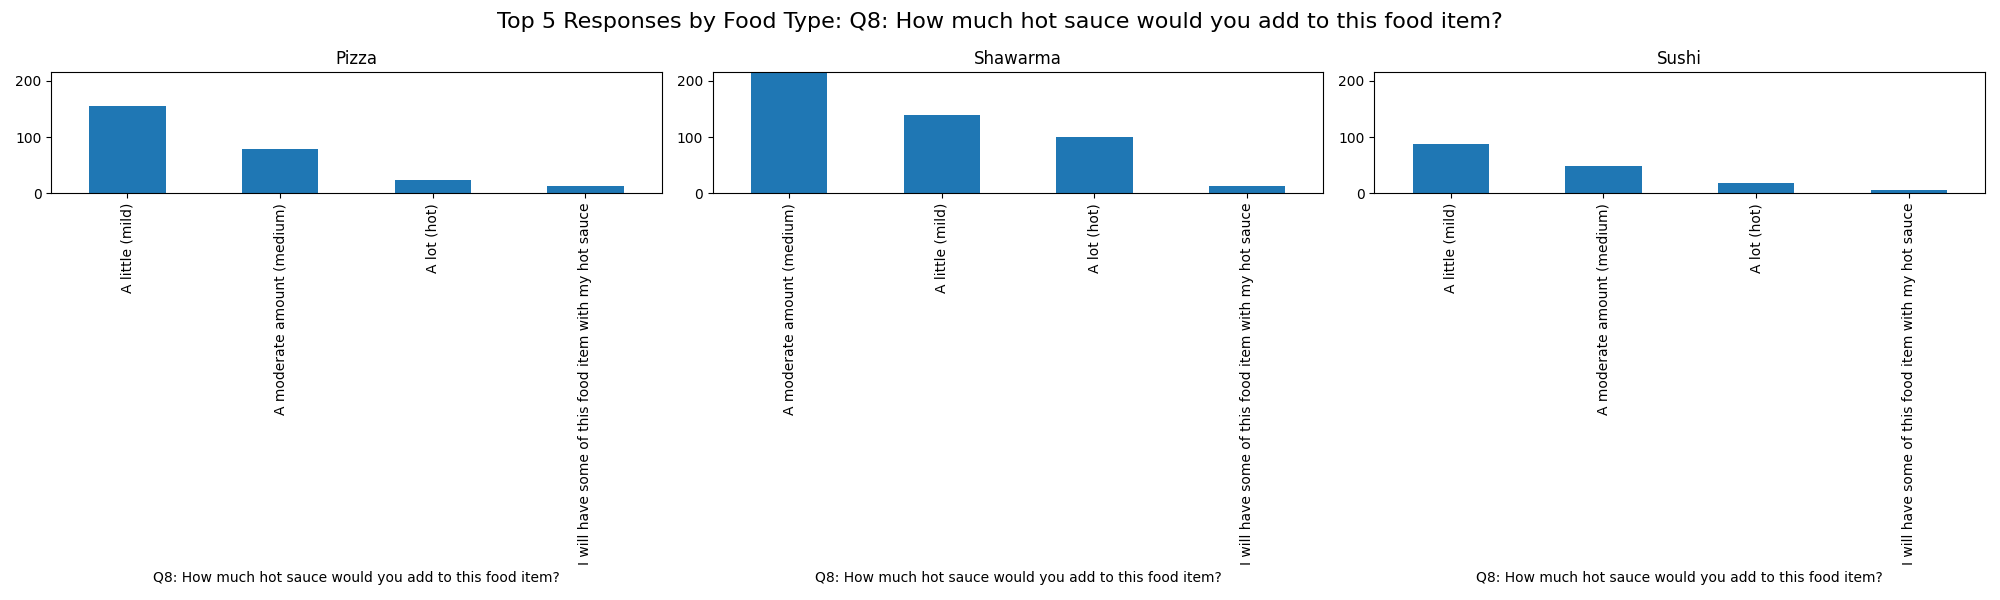
\includegraphics[width=\columnwidth]{data/top_5_responses_Q8.png}}
    \caption{Top 5 Responses for Q8}
    \label{f:q8}
\end{figure}




